\chapter{Introducción}

\section{Motivación y contexto}

El Programma 101 es considerado por muchos como el primer ordenador de uso
personal. Producido por la empresa italiana Olivetti entre los años 1962 y 1964,
este dispositivos seasimilaba más a una calculadora que al concepto de ordenador
que se tiene en la actualidad. Casi 60 años después, los ordenadores han
evolucionado hasta convertirse en un objeto asequible y casi indispensable,
teniendo la mayor parte de la sociedad acceso a algún dispositivo con capacidad
de computación. Aspectos de nuestra vida como el ocio, serían muy diferentes sin
las redes sociales o los servicios online. Esta evolución de los ordenadores y
la computación en general continúa hoy en día, buscando conectar dispositivos
cotidianos a internet e incorporar en ellos cierta capacidad de procesamiento.
Televisores inteligentes en los que instalar aplicaciones, robots aspiradores
que funcionan de manera autónoma, frigoríficos que permiten ver el estado de los
alimentos que almacenan, todos estos productos surgen de la expansión de los
ordenadores hasta todos los rincones de nuestras vidas, con el objetivo final de
hacerla más sencilla para los humanos. Esta expansión no está ocurriendo solo en
los hogares, si no que se avanza hacia un mundo más conectado donde
aparentemente todo lo que nos rodea tenga acceso a la red.

La industria no es ajena a este cambio, ya que la aplicación del internet de las
cosas (IoT por sus siglas en inglés) a los procesos industriales podría aportar
beneficios muy importantes como son el aumento de la productividad, de la
calidad de los productos o de la seguridad de las instalaciones. No obstante, se
trata de un proceso de implantación complejo y de muy largo plazo, debido a los
estrictos requisitos de algunos sectores industriales. Las fábricas y plantas de
producción relegan las tareas de control de sus operaciones a los sistemas de
control industriales o ICSs (\textit{Industrial Control Systems}). Normalmente,
estos sistemas deben responder ante eventos que ocurren en las instalaciones en
ventanas de tiempo muy pequeñas, dependiendo del proceso concreto y sus riesgos
asociados. La fiabilidad de estos sistemas y su tolerancia ante los fallos es de
gran importancia, siendo crucial la verificación de estos aspectos durante su
diseño y desarrollo. Es por estos requisitos tan estrictos que, en muchos casos,
para la implantación de los ICSs se utilizan tanto \textit{hardware} como
\textit{software} específicos y que ya han sido validados para este tipo de
aplicaciones. No obstante, el uso de estas herramientas también plantea algunos
inconvenientes, como por ejemplo la difícil interoperabilidad con otros sistemas
debido a la naturaleza cerrada de las mismas o la reutilización del código en
otras plataformas, lo que acorta la vida útil del \textit{software}.

Desde esta situación se afronta el avance hacia la cuarta revolución industrial
o Industria 4.0. Uno de los objetivos principales que se persigue es la
automatización completa de los procesos industriales, haciando que sean
independientes y autogestionados, aumentando así su eficiencia, productividad y
seguridad. Para conseguir este objetivo, es necesario incorporar a estos
procesos las nuevas técnicas de aprendizaje automático y análisis de grandes
volúmenes de datos, construyendo sistemas experots capaces de tomar decisiones
propias para su funcionamiento y gestión (p. ej., modificar el ritmo de
producción en base a predicciones sobre la demanda). Aunque estos sistemas
expertos se podrían desplegar en plataformas separadas de las que habitan los
ICSs, esto duplica los costes de infraestructura y hace también más difícil el
mantenimiento de la misma. Por ello, hay una tendencia cada vez mayor hacia la
ejecución de tareas con distintos niveles de criticalidad en una misma
plataforma. Por otra parte, las tareas de aprendizaje máquina suelen requerir de
una capacidad de computación relativamente elevada, sobre todo cuando la
cantidad de datos sobre la que se trabaja es grande. Un solo dispositivo no
sería capaz de gestionar estas tareas de forma eficiente si, además, debe
realizar tareas críticas de control, dificultando también que pueda cumplir con
sus requisitos en ese aspecto. Aparecen entonces nuevos paradigmas de
computación, como el \textit{fog} o el \textit{edge computing}, que pretenden
decentralizar el procesamiento, alejándolo de la nube y llevándolo a elementos
intermedios más cercanos a las fuentes de datos o a los dispositivos del borde
de la red, respectivamente. En estos paradigmas, se persigue la máxima
utilización de la capacidad de computación de los dispositivos presentes en la
red, distribuyendo entre ellos las tareas necesarias de forma dinámica.

Dentro de este campo, se están llevando a cabo muchas investigaciones para
validar la efectividad de estos nuevos modelos y hacerlos realidad, además de
comprobar su efectividad en el ámbito industrial. Uno de los planteamientos más
prometedores es el que conlleva la aplicación de tecnologías de virtualización a
los sistemas de control industrial, permitiendo su despliegue y ejecución
distribuida en convivencia con otros procesos. Estas tecnologías, que han
sufrido un desarrollo masico en los últimos años debido al auge de la
computación en la nube, pueden ahora ser claves para asegurar la resiliencia y
robustez de los ICSs en entornos distribuidos.

Por todo esto, este trabajo abordará la complejidad de los problemas descritos
intentando buscar mecanismos que simplifiquen la gestión de los sistemas
\textit{fog}/\textit{edge}. Partiremos de la experiencia previa en trabajos con
contenedores orientados al análisis de sus prestaciones para la ejecución de
tareas con restricciones temporales, responsables de las ideas aquí propuestas y
base fundamental de parte de la motivación de este trabajo. Además, esta línea
de investigación tiene mucho potencial para mejorar los sistemas de control
implementados en la actualidad, permitiendo por tanto una contribución
importante tanto en aspectos industriales como científicos, lo que aumenta aún
más nuestro interés en esta temática.

\section{Objetivos}

De cara a la realización de este trabajo, se han planteado los siguientes
objetivos a cumplir:

\begin{itemize}
      \item Comprender los conceptos básicos sobre sistemas operativos de tiempo
            real, algoritmos de planificación y sistemas de control industriales.
      \item Analizar las soluciones de tiempo real basadas en GNU/Linux existentes.
      \item Estudiar la viabilidad y rendimiento de las tecnologías de
            contenerización para la ejecución de tareas con restricciones temporales.
      \item Diseñar e implementar una herramienta de despliegue de tareas de
            tiempo real mediante contenedores que sirva como prueba de concepto.
      \item Caracterizar las prestaciones de la herramienta desarrollada,
            identificando posibles aplicaciones y/o mejoras de la misma.
\end{itemize}

Una parte relevante de los objetivos del presente proyecto están asociados al
estudio y caracterización de tecnologías, así como al análisis del mercado, que
se justifica por un enfoque innovador orientado al desarrollo de sistemas para
\textit{fog computing}. Esto, junto con los conocimientos adquiridos sobre
implementación de sistemas de tiempo real, será clave para que la herramienta
desarrollada como prueba de concepto sea lo más eficiente y funcional posible.

Por otra parte, en los objetivos también se hace hincapié en el uso de
soluciones basadas en GNU/Linux, como parte de un fuerte compromiso con las
herramientas libres y de código abierto. Algunos de los sistemas operativos de
tiempo real más conocidos y usados son de código propietario y es necesario
adquirir licencias para utilizarlos, lo cual no favorece ni el aprendizaje ni la
reutilización del software desarrollado para estas plataformas. Últimamente, se
han realizado contribuciones importantes al kernel de Linux para mejorar el
soporte que ofrece a cargas de trabajo de este tipo, además de los múltiples
proyectos más especializados que está llevando a cabo la comunidad. En esta
aproximación, hemos considerado primordial la extensión del software libre,
apoyando su uso siempre que sea posible. Por ello, la herramienta planteada se
diseñará en torno al despliegue de tareas en sistemas GNU/Linux.

\section{Planificación}

Tradicionalmente, la planificación de las tareas en proyectos de desarrollo de
software se realizaba siguiendo un modelo en cascada, donde antes de avanzar a
la siguiente fase (p. ej., diseño, desarrollo, prueba) se debían completar todas
las tareas de la anterior. Además, se intentaba estimar con precisión el tiempo
necesario para desarrollar cada tarea, con el fin de obtener una predicción
precisa de cúando estaría terminado el proyecto. Este tipo de metodología en
cascada, en la que se planifica la totalidad del proyecto de antemano, es muy
rígida y, por tanto, hace que sea más difícil adaptarse a los cambios que
suceden durante el desarrollo del proyecto. En los últimos años ha cobrado
fuerza una alternativa: las metodlogías ágiles. Lo que se plantea es afrontar la
planificación y ejecución de las tareas de forma iterativa. En SCRUM, una de las
metodologías ágiles más conocidas, se eligen tareas a realizar a corto plazo, lo
que permite modificar las tareas a realizar si fuera necesario. En
\cite{casteren_waterfall_2017} se realiza una comparativa entre el modelo en
cascada y las metodologías ágiles, llegando el autor a la conclusión de que
estas últimas son siempre más eficaces para proyectos de pequeño y medio tamaño
si se aplican de forma correcta. Es en los proyectos más complejos, donde hay
múltiples equipos involucrados, en los que la aplicación de metodologías ágiles
es más difícil y puede resultar ineficaz.

Observando esto y sabiendo que este proyecto es de baja complejidad, hemos
decidido aplicar SCRUM para la planificación y la gestión de las tareas del
mismo. Según este modelo, el desarrollo del proyecto se realiza en iteraciones,
las cuales se planifican de forma dinámica y sobre la marcha. Al inicio del
proyecto, se identifican las tareas que se consideran necesarias para la
consecución de los objetivos, formando una pila o \textit{backlog} de tareas.
Los miembros del equipo estiman estas tareas en base a su experiencia. A
diferencia del modelo tradicional, estas estimaciones no tienen que ser
precisas, sino que lo que se busca es una medida orientativa del tamaño o
complejidad de las tareas en relación con las demás. En muchos casos, para
agilizar el proceso de estimación, se aplican juegos. Una vez definida esta pila
de tareas, comienzan las iteraciones o \textit{sprints}, que suelen tener una
duración pequeña, de 2 o 3 semanas. Antes de comenzar una nueva iteración, los
miembros del equipo deciden qué tareas se van a acometer en la misma. La
selección de estas tareas se puede basar en su estimación, su importancia o en
el propio deseo de los miembros del equipo de realizarlas. Así, se realiza una
planificación a corto plazo, lo que permite a los equipos tener mucho margen de
reacción ante cambios en el proyecto (p. ej., cambios en los requisitos o
problemas imprevistos). Una vez termina la iteración, el equipo evalúa el
trabajo realizado, comprobando si las estimaciones que habían realizado al
principio eran fidedignas, actualizando las de las tareas restantes si fuera
necesario. Si se ha descubierto que se deben realizar más tareas de las
inicialmente planteadas, éstas se pueden añadir a la pila entre iteraciones.

Como se puede apreciar, el modelo de SCRUM se centra mucho en el trabajo
colaborativo dentro del equipo, por lo que el modelo que hemos aplicado en este
proyecto se puede considerar como un SCRUM adaptado al trabajo individual. Las
iteraciones seguidas han sido de dos semanas y se ha usado un tablero Kanban
para el seguimiento de las tareas. En la figura \ref{fig:01-kanban} se muestra
el tablero usado. El objetivo de estos tableros es ofrecer una visión clara del
estado del proyecto con un simple vistazo, para lo que ordenan las tareas en
tres columnas: Por hacer (\textit{To do}), Haciendo (\textit{In progress}) y
Hecho (\textit{Done}). A continuación, se listan las iteraciones realizadas con
las tareas que se han acometido en cada una de ellas:

\begin{figure}
      \centering
      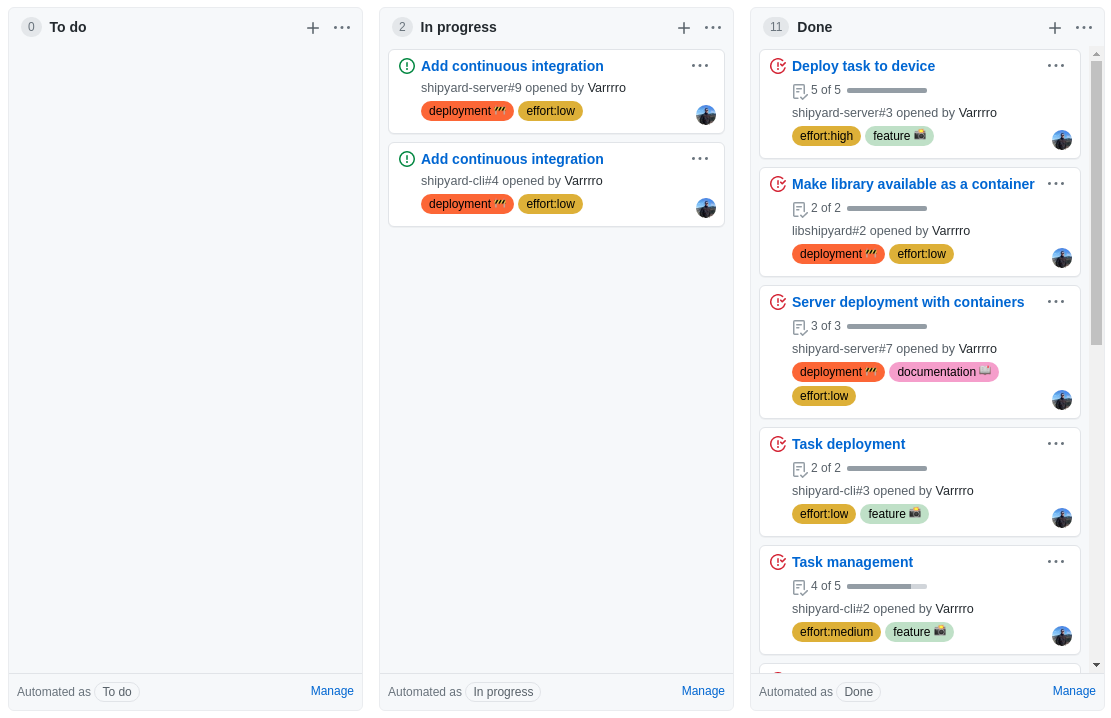
\includegraphics[width=\textwidth]{01-introduction/kanban.png}
      \caption{Muestra del tablero Kanban usado para el seguimiento de las tareas del proyecto}
      \label{fig:01-kanban}
\end{figure}

\begin{itemize}
      \item \textbf{Iteración 1} (06/07 - 20/07)
            \begin{itemize}
                  \item (Documentación) Estudiar el funcionamiento de los RTOS.
                  \item (Documentación) Estudiar las soluciones de tiempo real
                        para Linux.
                  \item (Documentación) Estudiar las técnicas de diseño e
                        implementación de tareas de control.
                  \item (Documentación) Estudiar el uso de contenedores para
                        tareas de tiempo real.
            \end{itemize}
      \item \textbf{Iteración 2} (20/07 - 03/08)
            \begin{itemize}
                  \item (Servidor) Implementar la obtención, inserción y
                        eliminación de nodos.
                  \item (Servidor) Implementar la obtención, inserción y
                        eliminación de tareas.
            \end{itemize}
      \item \textbf{Iteración 3} (03/08 - 17/08)
            \begin{itemize}
                  \item (Servidor) Implementar el despliegue y la eliminación de
                        tareas en los nodos.
            \end{itemize}
      \item \textbf{Iteración 4} (17/08 - 31/08)
            \begin{itemize}
                  \item (Servidor) Implementar la obtención, inserción y
                        eliminación de tareas.
                  \item (Servidor) Implementar el despliegue y la eliminación de
                        tareas en los nodos.
                  \item (Servidor) Implementar la actualización de nodos y
                        tareas.
                  \item (Librería) Implementar las funciones de manipulación de
                        los atributos de planificación.
                  \item (Librería) Crear imagen base.
            \end{itemize}
      \item \textbf{Iteración 5} (31/08 - 14/09)
            \begin{itemize}
                  \item (Servidor) Mejorar el manejo de los errores.
                  \item (Servidor) Definir despliegue mediante contenedores.
                  \item (Cliente) Implementar la gestión de los nodos.
                  \item (Cliente) Implementar la gestión de las tareas.
                  \item (Cliente) Implementar el despliegue de tareas.
            \end{itemize}
      \item \textbf{Iteración 6} (14/09 - 28/09)
            \begin{itemize}
                  \item (Servidor) Implementar el despliegue y la eliminación de
                        tareas en los nodos.
                  \item (Cliente) Implementar la gestión de los nodos.
                  \item (Cliente) Implementar el despliegue de tareas.
                  \item (Librería) Implementar las funciones de manipulación de
                        los atributos de planificación.
                  \item (Librería) Crear imagen base.
            \end{itemize}
      \item \textbf{Iteración 7} (28/09 - 12/10)
            \begin{itemize}
                  \item (Experimentación) Caracterizar el impacto de los
                        contenedores sobre el rendimiento en tareas de tiempo
                        real.
            \end{itemize}
      \item \textbf{Iteración 8} (12/10 - 26/10)
            \begin{itemize}
                  \item (Experimentación) Caracterizar el impacto de los
                        contenedores sobre el rendimiento en tareas de tiempo
                        real.
            \end{itemize}
      \item \textbf{Iteración 9} (26/10 - 09/11)
            \begin{itemize}
                  \item (Experimentación) Caracterizar el rendimiento del
                        sistema desarrollado.
            \end{itemize}
      \item \textbf{Iteración 10} (09/11 - 23/11)
            \begin{itemize}
                  \item (Servidor) Definir flujo de integración continua.
                  \item (Cliente) Definir flujo de integración continua.
                  \item (Librería) Definir flujo de integración continua.
            \end{itemize}
\end{itemize}

Como se puede apreciar, las tareas se han diferenciado según su tipo o el
componente del sistema desarrollado al que se refieren. Además, para algunas de
estas tareas ha sido necesario dedicar más de una iteración. En el caso de la
tarea de implementación de las operaciones de obtención, inserción y eliminación
de tareas, se tuvo que volver a incorporar en la iteración 4 debido a algunos
errores cometidos en la implementación y que se detectaron más tarde. Otro caso
similar fue la implementación de la funcionalidad de despliegue de tareas en los
nodos. En el código inicialmente escrito en las iteraciones 3 y 4, esta
operación se llevaba a cabo abriendo directamente una conexión SSH con el nodo
objetivo y ejecutando los comandos de despliegue, emulando lo que haría un
operario humano. Posteriormente, se llegó a la conclusión de que esta
implementación se podía mejorar la usar la librería oficial de Docker para
Python, con la cuál se podía establecer una conexión al motor Docker del nodo
remoto para realizar el despliegue. Estas situaciones, junto con otras dadas en
más tareas, reflejan fielmente la capacidad de adaptarse a los imprevistos que
ofrece SCRUM que ya hemos comentado anteriormente.

\section{Material y métodos}
\label{sec:01-tools}

En esta sección, se presentan todas las herramientas que se han usado para
llevar a cabo este proyecto, además de las metodologías de trabajo seguidas. En
la figura \ref{fig:01-tools} se puede ver una recopilación de los logotipos de
todas estas herramientas, las cuales se van a exponer en detalle a continuación.

En un proyecto de desarrollo de código como es este, una de las herramientas más
importantes es la de control de versiones. En nuestro caso, se ha usado
\textbf{Git} debido a que es una herramienta de código libre y, además, es la
más conocida y usada. El repositorio remoto se ha alojado en \textbf{GitHub}, la
popular plataforma de desarrollo de código colaborativo. El desarrollo de código
como tal se ha hecho con \textbf{Visual Studio Code}, un editor de texto de
Microsoft que, aunque ofrece menos funcionalidad de serie que los entornos de
desarrollo (IDEs) especializados, también es mucho más liviano y rápido. Además,
esta funcionalidad se puede extender enormemente mediante extensiones, pudiendo
convertirlo casi en un IDE adaptado a las necesidades concretas del usuario.
Gracias a estas extensiones, se puede usar el mismo editor para distintos
programar en distintos lenguajes, lo cual ha sido una de las principales razones
por las que se ha escogido.

\begin{figure}[H]
      \centering
      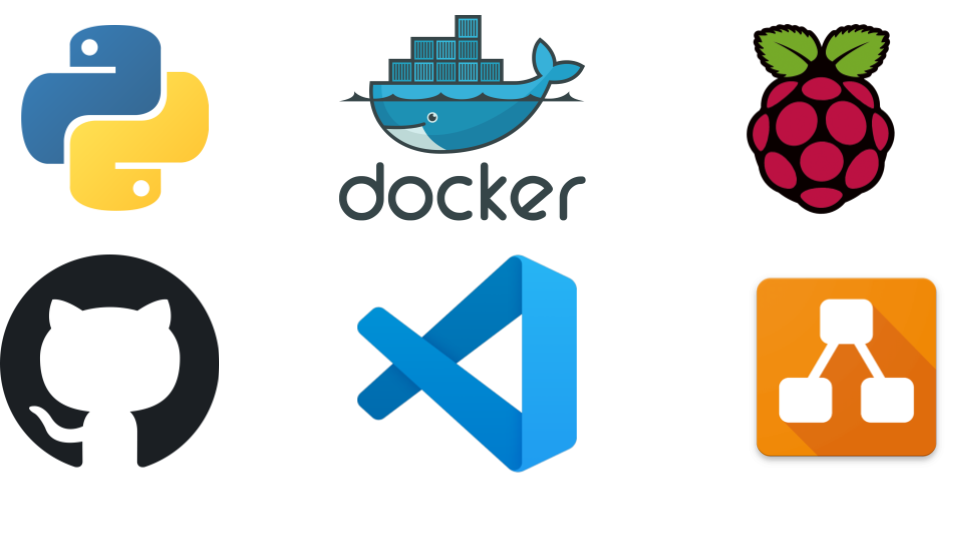
\includegraphics[width=0.7\textwidth]{01-introduction/tools.png}
      \caption{Logotipos de las herramientas utilizadas. De izquierda a derecha y%
            de arriba a abajo: Python, Docker, Raspberry Pi, GitHub, VS Code y
            draw.io}
      \label{fig:01-tools}
\end{figure}

Como ya se ha indicado en la sección anterior, se ha aplicado un SCRUM adaptado
como metodología de planificación, gestión y seguimiento del proyecto, usando un
tablero Kanban para la visualización de las tareas. Concretamente, se ha usado
el tablero que ofrece GitHub como parte de sus herramientas para la gestión de
proyectos. Las tareas se añaden a los repositorios como \textit{issues}, los
cuales se añaden al tablero para controlar su estado de realización. El
beneficio que nos aporta el uso de GitHub para esto es el de tener una
plataforma unificada tanto para la gestión del proyecto como para su desarrollo.
Esta integración permite flujos de trabajo muy interesantes, como por ejemplo
referenciar los \textit{issues} ya mencionados en los mensajes de
\textit{commit}, de forma que se vinculan los cambios realizados con la tarea en
la que se engloban. La gestión del proyecto es, por tanto, más directa y
sencilla.

Además del tablero de proyecto y los propios repositorios de Git, también se ha
hecho uso de \textbf{Actions}, la herramienta de CI/CD de GitHub. Como su propio
nombre indica, se definen acciones en flujos de trabajo que se ejecutan para los
eventos del repositorio (p. ej., un nuevo \textit{push}, la publicación de una
nueva versión del producto, un \textit{pull request}) que desee el
desarrollador. Estas acciones pueden incluir, por ejemplo, la ejecución de
pruebas, la construcción de artefactos o el despliegue del software sobre
diversas plataformas. Así, se consigue automatizar los procesos de despliegue y
se incorporan también medidas para el control de la calidad del código. En
nuestro caso, en la ejecución de las pruebas se genera un informe sobre la
cobertura del código, el cuál se envía a \textbf{Codecov}, una plataforma
especializada en este tipo de informes, para su análisis y visualización.

Los diagramas que se presentan a lo largo de este trabajo, incluidos los que
componen el diseño de la herramienta desarrollada y sus componentes, se han
creado con la herramienta online \textbf{draw.io}. Al integrarse directamente
con Google Drive, se puede usar desde el navegador, siendo una solución muy
cómoda y accesible para la creación de estos diagramas.

En cuanto al desarrollo y despliegue de la herramienta planteada, se han
utilizado varias tecnologías. Los lenguajes de programación son Python y C, muy
conocidos y utilizados en la industria. C es el lenguaje de referencia para la
programación de sistemas y las tareas de bajo nivel, mientras que Python ofrece
una sintaxis muy sencilla para la implementación de herramientas como
aplicaciones o servidores. Python también posee una nutrida colección de
librerías para distintos casos de uso, lo cual también fue muy atractivo para su
elección. En este proyecto, se usan varias de estas librerías para facilitar la
implementación de algunos aspectos de la herramienta. Destacamos las siguientes:

\begin{itemize}
      \item \textbf{hug} - Escritura de APIs sencilla y sin ataduras. Esta
            librería trata de competir con otras más conocidas como Flask, proponiendo
            un modelo mucho más simple y dando más libertad al desarrollador.
      \item \textbf{click} - Más que una librería, se trata de un
            \textit{framework} para la implementación de aplicaciones de línea de
            comandos (CLI). Ofrece todas las utilidades que se pueden necesitar para
            este tipo de aplicaciones, como es la generación automática de páginas de
            ayuda.
      \item \textbf{marshmallow} - Esta librería permite la sencilla
            deserialización y serialización de objetos JSON a objetos Python. Esto es
            especialmente útil al trabajar con servicios web, ya que se pueden leer los
            datos JSON recibidos y validarlos frente a un esquema de datos definido por
            el desarrollador.
      \item \textbf{pymongo} - Ejecución de consultas sobre bases de datos
            MongoDB, que son las usadas en este proyecto.
      \item \textbf{paramiko} - Herramientas para trabajar con SSH desde Python.
            Esencial para el despliegue de las tareas sobre los nodos.
      \item \textbf{docker} - La librería oficial de Docker para Python. Con ella,
            se puede conectar con un servidor Docker (local o remoto) para ejecutar
            operaciones de construcción de imágenes o lanzamiento de contenedores.
      \item \textbf{requests} - Es la librería más conocida para la realización de
            peticiones HTTP en Python.
      \item \textbf{unittest} - Aunque no se trata de una librería externa como
            las demás, ya que forma parte de la librería estándar de Python, merece ser
            destacada por ser la utilizada para la escritura y ejecución de las pruebas
            del código desarrollado.
\end{itemize}

Además de estas librerías, se han usado otras para el análisis y formateo del
código como son \textbf{pylint} y \textbf{autopep8}.

Como ya se ha mencionado, la herramienta desarrollada trabaja con
\textbf{MongoDB} para la gestión del almacenamiento persistente de los datos y
el acceso a los mismos. Se trata de un gestor de bases de datos documental que
pertenece a la familia NoSQL (\textit{Not only SQL}). Las bases de datos
documentales divergen del modelo relacional tradicional que siguen otros
gestores tan famosos como MySQL o PostgreSQL. No existen los conceptos de tabla
o fila, sino que se almacenan colecciones de documentos no estructurados. En el
caso de MongoDB, se trabaja con documentos JSON, formato ampliamente usado en el
entorno web para la transmisión de datos debido a su legibilidad y velocidad de
serialización/deserialización. Cuando decimos que los documentos son no
estructurados, nos referimos a que no tienen por qué poseer los mismos campos,
ya que no hay un esquema definido a seguir. MongoDB no cumple con ACID, pero es
una pérdida aceptable a cambio de la flexibilidad y facilidad de uso que nos
ofrece. Además, el lenguaje de consultas es mucho más claro e intuitivo que SQL,
permitiendo realizar consultas de envergadura similar.

La idea principal en torno a la cual gira este trabajo es la del uso de
contenedores para el despliegue de tareas de tiempo real. En este sentido,
\textbf{Docker} es la tecnología de contenerización en la que nos hemos apoyado
para la implementación de la herramienta propuesta. Esta elección recae
principalmente en el hecho de que se trata del motor de contenedores más
conocido y utilizado. De la mano de Docker, también se ha utlizado
\textbf{Docker Compose} para el despliegue sencillo de un entorno de desarrollo
completo que permita replicar un despliegue de producción de forma simplificada.
Las imágenes de contenedores definidas en este proyecto, se han alojado en el
repositorio de imágenes \textbf{DockerHub}, aprovechando que proporciona un
sistema de construcción automática de imágenes.

\begin{figure}
      \centering
      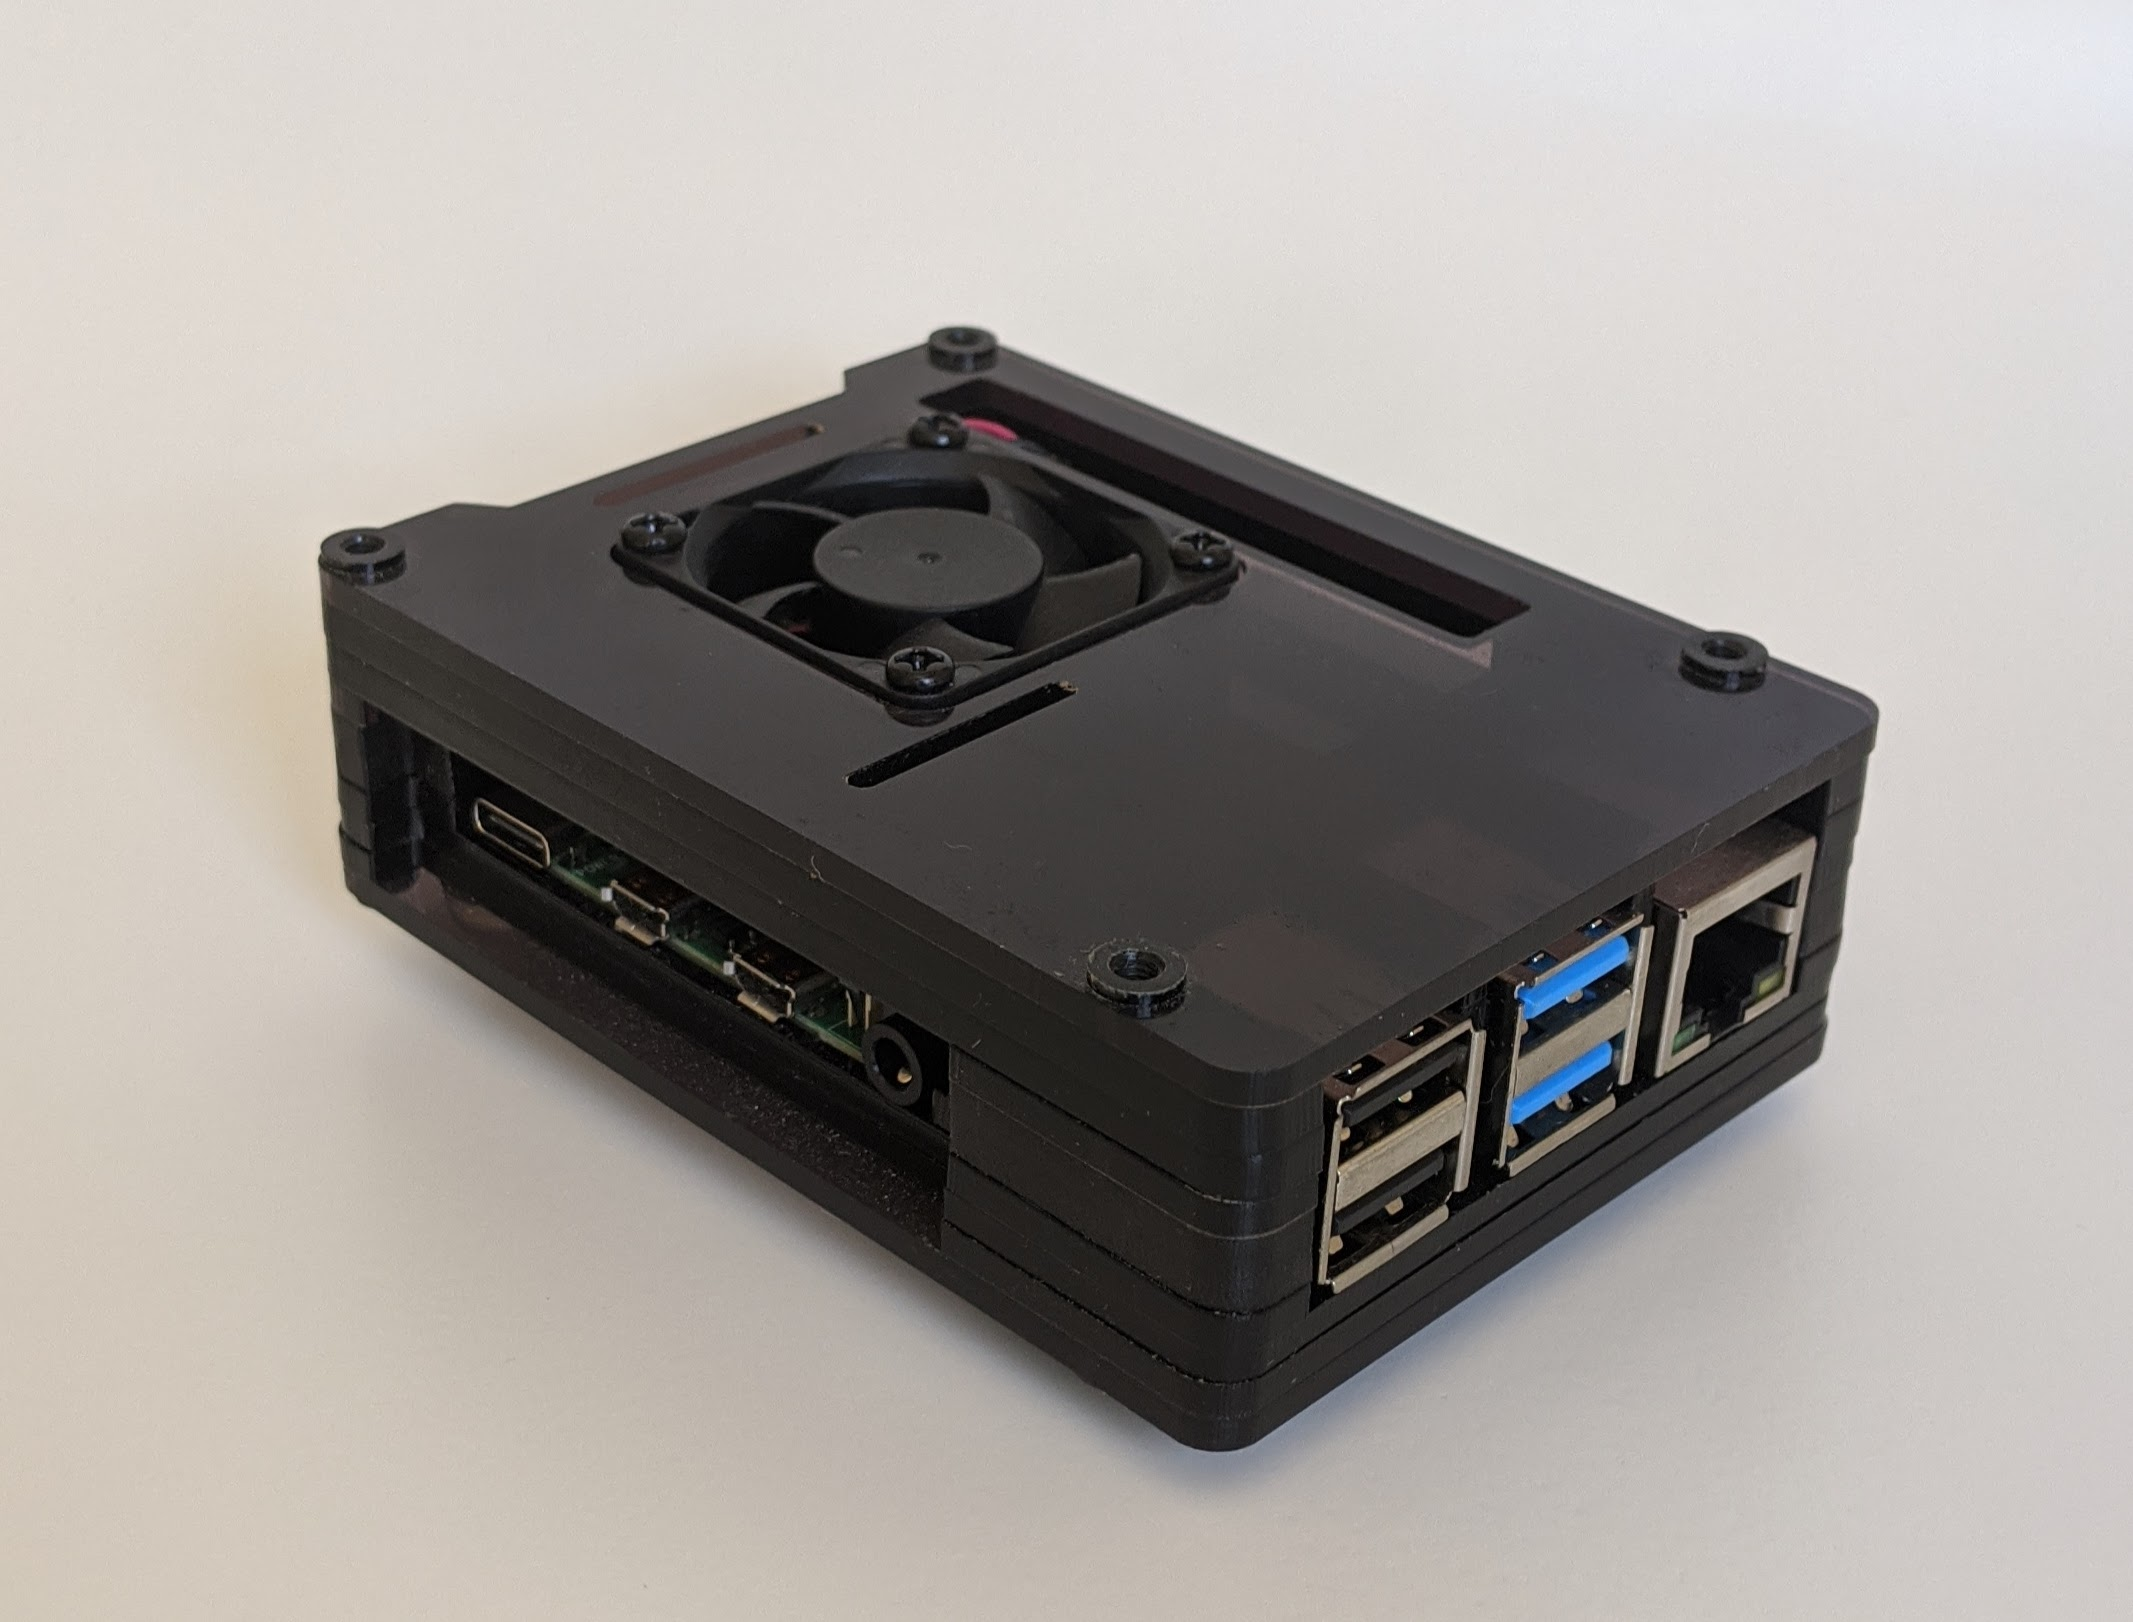
\includegraphics[width=0.8\textwidth]{01-introduction/raspberry-pi.jpg}
      \caption{Raspberry Pi 4B utilizada en el trabajo}
      \label{fig:01-raspberry_pi}
\end{figure}

Para realizar las pruebas del sistema desarrollado, se ha usado una
\textbf{Raspberry Pi 4B}, concretamente la que se muestra en la figura
\ref{fig:01-raspberry_pi}. Se trata de un SBC (\textit{Single Board Computer})
de bajo coste y muy versátil, pudiendo usarse para infinidad de aplicaciones.
Las características detalladas de esta plataforma se pueden ver en la tabla
\ref{tab:01-raspberry_specs}.

\begin{table}[H]
      \centering
      \begin{tabular}{ |>{\columncolor[gray]{0.8}}l|p{0.5\textwidth}| }
            \hline
            \textbf{Procesador}          & Cortex-A72                \\
            \hline
            \textbf{Arquitectura}        & ARMv7                     \\
            \hline
            \textbf{Número de núcleos}   & 4                         \\
            \hline
            \textbf{Frecuencia de reloj} & 1500 MHz                  \\
            \hline
            \textbf{RAM}                 & 4 GB                      \\
            \hline
            \textbf{Sistema operativo}   & Raspberry Pi OS Lite 4.19 \\
            \hline
      \end{tabular}
      \caption{Especificaciones de la Raspberry Pi usada en el trabajo}
      \label{tab:01-raspberry_specs}
\end{table}

El sistema operativo de este dispositivo es GNU/Linux (concretamente, basado en
Debian), al que se le ha aplicado la revisión 24 del parche de tiempo real
\texttt{PREEMPT\_RT}. Este parche aporta al sistema la capacidad de realizar
planificación de procesos apropiativa. En el apéndice
\ref{app:03-container_tests} se explica con detenimiento el proceso seguido para
usar el kernel de Linux con \texttt{PREEMPT\_RT} en la Raspberry Pi.

\section{Estructura de la memoria}

En el capítulo 1, se ha introducido el proyecto y explicado tanto la motivación
detrás del mismo como los objetivos planteados, la planificación seguida y las
herramientas, tecnologías y metodologías que se han utilizado.

En el capítulo 2, se realiza un estudio en profundidad del estado de la técnica
en lo relativo a los sistemas confiables, la computación en la nube y sus
derivados, las tareas de tiempo real y las tecnologías de virtualización. Se
introducen todos los conceptos relevantes, además de presentar otros trabajos
interesantes llevados a cabo en estas áreas.

En el capítulo 3, se analiza el rendimiento de los procesos de tiempo real
contenerizados, haciendo especial hincapié en el impacto que tienen sobre el
mismo las tecnologías de contenerización frente a procesos no virtualizados.

En el capítulo 4, se aborda el diseño de una herramienta para el despliegue y
seguimiento de tareas de tiempo real en entornos distribuidos, así como su
implementación y prueba. Se presentan los resultados obtenidos y se discute
sobre los mismos.

En el capítulo 5, se realiza una revisión del proyecto completo y se presentan
las conclusiones, así como las maneras en las que se puede extender y mejorar el
trabajo realizado.
